\documentclass[10pt,a4paper]{article}
\usepackage[utf8]{inputenc}
\usepackage{amsmath}
\usepackage{amsfonts}
\usepackage{amssymb}
\usepackage{graphicx}
\begin{document}


We need to communicate with the mars rover over large distances. This will be, of course, scaled down to reasonable distances on earth for the challenge. To make communication possible we will look into the theory first in the form of a link budget analysis and the hardware part which is mainly our two transceivers. One on the mars rover itself, and one on the user side. Therefor this part is not specifically mentioned in both parts but mentioned here in the report.

\subsection{Link budget analysis}
For communications from point to point we need to do a Link Budget Analysis.

\begin{figure}[!h]
    \centering
    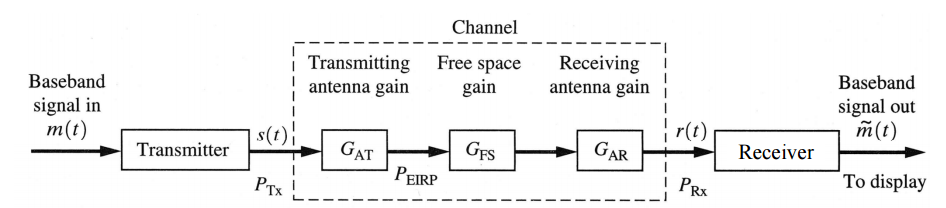
\includegraphics[scale=0.6]{figures/LinkBudget.png}
    \caption{Link Budget Analysis}
\end{figure}

Here the Transmitter will send a modulated signal, which at the receiver side will be influenced by a couple of factors. The $P_{tx}$ is the output power by the sender, and $P_{EIRP}$ is the total power including the antenna gain transmitted by the sender. After transmitting we will lose power, we call this the free space gain $G_{FS}$. we can calculate the power at the output of the receiving antenna $P_{rx}$ according to Equation \ref{Overallpowergain}. Note that all the variables are in dB in this equation.

\begin{equation}
\label{Overallpowergain}
(P_{Rx})_{dB} = G_{AT} + G_{FS} + G_{AR} + P_{Tx}
\end{equation}
\subsubsection{Antenna gain}
The antenna gain is approximated by Equation \ref{EffectiveArea}.
\begin{equation}
\label{EffectiveArea}
G_{A} = \frac{4 \pi A_e}{\lambda^2}
\end{equation}

With this approximation we can view different Antenna options, with the gains in the table below.
\begin{table}[!h]
\caption {Antenna gains and effective area's}
\center 
\begin{tabular}{l*{2}{c}r}
Antenna Type      & $G_A$ & $A_e$ \\
\hline
Isotropic 				& 1 & $\lambda^2$/4$\pi$ \\
Half-wave dipole        & 1.64 & 1.64$\lambda^2$/4$\pi$ \\
Horn, mouth area A      & 10A/$\lambda^2$ & 0.81A \\
Parabola, face area A   & 7A/$\lambda^2$ & 0.56A \\
\end{tabular}
\end{table}

As we see the Isotropic antenna has a gain of 1, this is because it sends an equal amount of $P_{Tx}$ in all directions thus the isotropic antenna is used as a reference for the antenna gains.

\subsubsection{Free space gain}
The free space gain is the gain that happens when the wave travels from point to point. We can calulate the free space gain $G_{FS}$ with equation \ref{Freespacegain}.

\begin{equation}
\label{Freespacegain}
G_{FS} = (\frac{\lambda}{4\pi d})^2
\end{equation}

Where $\lambda = c/f$ with c the speed of light which is approximately $3\cdot 10^8$. Since it is easier to work in dB de formula for the free space loss $(L_{FS})_{dB}$ we can write down the free space loss as following.

\begin{equation}
(L_{FS})_{dB} = 20 \log(\frac{4\pi d}{\lambda})dB
\end{equation}

\subsubsection{signal-to-noise ratio}
As showed in equation \ref{Overallpowergain} we can see that we will have a $P_{Rx}$ on the other side of the channel. Assuming we know the total noise temperature $T_{syst}$ of the receiver part of the system we can find out how much noise we will have at the output of our total system. This is related by equation \ref{totalnoise}

\begin{equation}
\label{totalnoise}
N=kT_{syst}B
\end{equation}

If we divide $P_{Rx}$ by N we have our SNR from which we can see if noise will become a problem when receiving data.

\subsection{Transceiver}
Our transceiver excists out of a load of components. We need an oscillator, a circuit that will handle our chosen modulation and a mixer. We will first handle list some oscillator choices. We can also choose to buy a complete package cointaining all the part or we decide to buy the parts apart, or even to build it ourselves. The signal that we have on the input of the Transceiver will be a digital signal already which is why we won't require any pulse amplitude modulation or sampling.
\subsubsection{Oscillator}
We can distinguish 3 different kind oscillators. A first order, second order and higher order oscillators. We can base this on the differential equation shown in equation \ref{diffequation}.
\begin{equation}
\label{diffequation}
f_1(x)\ddot{x} + f_2(x)\dot{x} + f_3(x) = 0
\end{equation}
A first order oscillator would then mean that we only have one dynamic time dependend element. The advantage of first oscillator is that it is it's tunability which might be a very wanted property since there might be other rovers communicating on our channel so we can easily switch the frequency. The downside of these oscillators is their stability. The stability however can be improved by making use of injection-locking of multiple first order oscillators. Second order oscillators have a great stability but their tunability is not that good. The last oscillator group is the third order and higher group which is not very stable since it is prone to chaos and not very tunable. The positive side is that it is relatively easy in design.

\subsubsection{Modulation}
When modulating we can choose between Amplitude Modulation (AM) and Frequency Modulation (FM). This will our first choice toward a modulation technique. When using an AM modulation technique we change the amplitude in a frequency to be able to transfer where when using FM we use frequency changes in order to transfer bits. The circuit used for each modulation technique differs from eachother which is why we will look into this after making a desicion. 
\end{document}